\section{Overview}

\begin{figure}[!t]
  \centering
  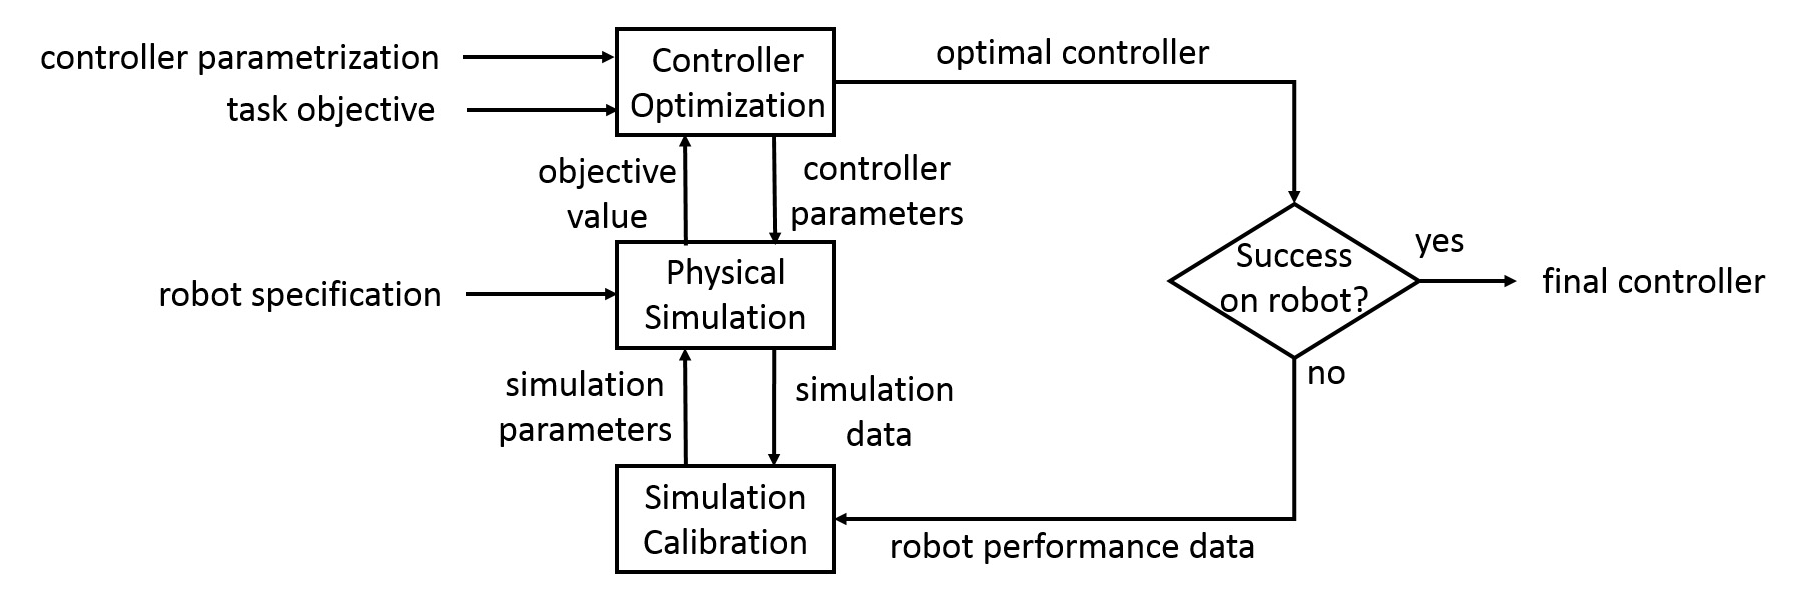
\includegraphics[width=0.5\textwidth]{figures/controllerTransfer}
  \caption{Overview of our algorithm.}
  \label{fig:controllerTransferOverview}
\end{figure}

We have developed a system that can automatically design locomotion controllers for robots (Figure~\ref{fig:controllerTransferOverview}). Given the specification of the robot, including its body shape, the physical properties of each body, and the types of joints, we build a physical simulation using Dynamic Animation and Robotics Toolkit (DART) \cite{dart:2012}. The controller optimization subsystem runs thousands of simulations to search for the optimal controller that maximizes the task-related fitness function. We then test this optimal controller on the robot. If the robot successfully completes the task, a working robotic controller is found and our algorithm terminates. Otherwise, we record the robot performance data and feed it into the simulation calibration subsystem. Simulation calibration runs another optimization, which searches for the optimal simulation parameters to minimize the discrepancy between the performance of the robot in the simulation and in the real world. The loop of controller optimization and simulation calibration is performed iteratively until the controller works successfully on the real robot. In the next three sections, we will present the algorithmic details of these components.
\karen{At some point, we need to discuss why we pick these tasks? Do we expect this system to work with walking/running?}
\jie{The logic sequence I am trying to convey is that we have the tasks first. They worth studying. Then we develop a system to achieve these tasks. All the tasks have a common theme: change between two postures while keep balance. We use four tasks that are quite different but fall in the same categorty to prove that our system is general. Whether this system will work on walking/running is beyond the scope of this paper. It is discussed in the future work section. }
